\section{Implementation}

In this section, we'll show how the first part of the algorithm is actually implemented.

As we said previosly, the objective of this part is to integrate the new instances and update the patterns.

The steps of the algorithm are the following:
\begin{itemize}
    \item When new labelled instances are passed, they are added to the existing instances.
    \item New patterns or \textit{shapelets} are computed 
    \item Each instance is assigned to a pattern 
    \item All the parameters for the modeling part are updated with respect to the new patterns
\end{itemize}

For the first part, not much has to be explained, the algorithm is called with the arguments 
\texttt{DL, L, Li}, which represent respectively the whole set of labelled instances, their labels and their
indexes.

At each iteration, the algorithm looks for new indices inside \texttt{Li} and adds them to the existing 
instances in the correct format, the instances are stored inside a dataframe with the following structure:
\begin{itemize}
    \item \texttt{key}: containing indices of the instances, in integer, datetime, or float format 
    \item \texttt{ts}: containing arrays with actual instances
    \item \texttt{label}: integer
    \item \texttt{near\_pt} : containing the key of the pattern each instance is assigned to
\end{itemize}

To compute new shapelets for the dataset, the algorithm makes use of two libraries: \texttt{pyts} and 
\texttt{sklearn}. In particular, we make use of the transformation module for the first and of the 
DecisionTree module for the second. 

First we compute the \textit{shapelet transform} of each labelled instance. This procedure finds a set of 
shapelets that might be useful to classify data inside the labelled instances, then, it calculates the distance
between the instances and each shapelet.

This operation is called \textit{shapelet transform}, since we transform each instance into a set of feature. 
Where each feature is the distance between the instance and each shapelet found. It is useful to say though that 
this transform \textit{does not substitute} the instances, but it's only an intermediate step.

Once the shapelet transform of each instance has been calculated, we need to find the most useful shapelets, that
will constitute our \textbf{patterns}.

To do this, we make use of a decision tree, from the library \texttt{sklearn}.

The decision tree acts on the shapelet transform of the data and finds the best splits according to the 
\textit{information gain}.

We can see an example in Figure (\ref{fig:tree}): each feature is a distance between
shapelet and instance. The first node splits on shapelet 18. 70 instances of the 
same label are grouped. They are assigned to shapelet 18, which will be the first
pattern found. A completely pure pattern.

Going down the tree, we apply the same logic to every leaf node, by assigning all 
the instances in it to the decision node just above.

Another example: there is a decision node which splits on feature 59, but it has
no leaf node, so no instance will be assigned to pattern 59.

In this way each instance is assigned to a pattern in order to maximize the 
information gain.

\begin{figure}
    \centering
    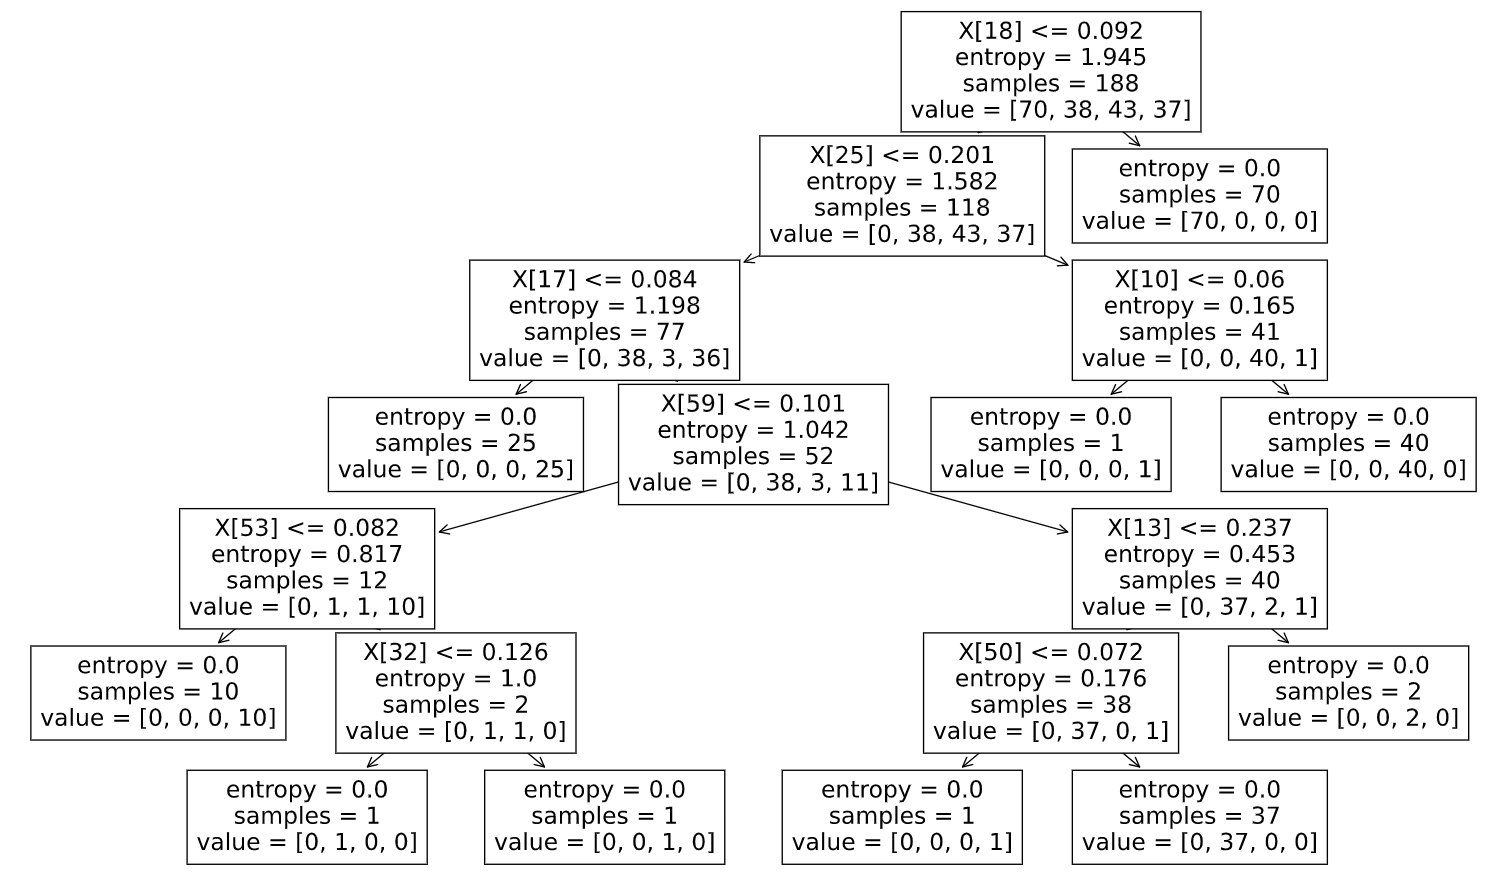
\includegraphics[width=0.80\textwidth]{tree.png}
    \caption{An example of tree structure acting on the shapelet transorms}
    \label{fig:tree}
\end{figure}

Once the patterns have been computed and each instance has been assigned to 
a certain pattern, we start the modeling part.

The objective is to calculate some useful parameters by MLE.

The first parameter is $\lambda$. The algorithm model the 
following probability with an exponential distribution:
\begin{equation}
    P(X_i | pt) = \exp(-\lambda_{pt} Dis(X_i, pt))
\end{equation}

Where $X_i$ is a time series and $pt$ is a pattern. $Dis$ is the distance 
function between the two.

We have a $\lambda$ parameter for each pattern, that we have to estimate via MLE.

The results are saved inside a the column \texttt{lambda} inside the pattern
dataframe. 

The second set of parameters to be estimated is the probabilities:
\begin{equation}
    P(pt | l) = Multi(p_1, \dots, p_l)
\end{equation}

Where \textit{multi} stands for multinomial. These parameters are also saved in a 
column of the patterns dataframe, called \texttt{l\_probas}.



